%本章では,提案手法である ID の連続性を意識した Sequential と
%演算時のアクセス局所性を意識した DBG Early Estimation (DBG-EE) についてそれぞれ説明する.
本研究では,グラフを取得しながらノード ID を再配置する手法として,Sequential と DBG Early Estimation (DBG-EE) を提案する.
図\ref{research_position} で示すように,Sequential は ID の連続性を意識し,DBG-EE は演算時のアクセス局所性を意識している.
Sequential では ID の連続性を保証するために RW で出会ったノード順に昇順の連続した ID を再配置する.
DBG-EE では 図\ref{degree_appro} で示すように,RW 途中での取得グラフにおける次数分布が RW 終了時点の取得グラフにおける次数分布に近似する性質に着目し ID を再配置する.
具体的には,既存手法でノードの次数情報しか必要とせず,前処理コストと演算速度向上のバランスに優れる DBG \cite{faldu2019closer} をもとに再配置を行う.
\begin{figure}[t]
  \centering
  %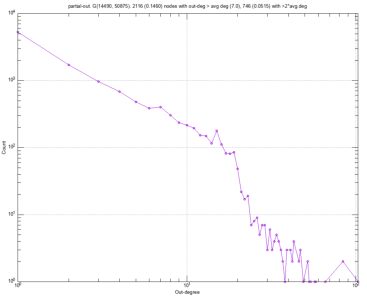
\includegraphics[width=\linewidth]{./figure/degree_appro.pdf}
  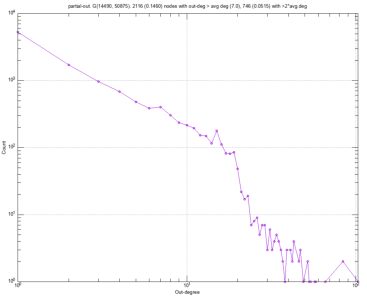
\includegraphics[width=12cm]{./figure/degree_appro.pdf}
  \caption{取得途中のグラフと取得完了時のグラフにおける次数分布}
  \label{degree_appro}
\end{figure}
\section{Sequential}
Sequential では,RW によるグラフ取得において新しく出会ったノード順に連続した昇順の ID を再配置する.
再配置に伴い新たな ID が割り振られる度に,元の ID と新たな ID の対応関係をマッピングテーブルへ登録する.
このマッピングテーブルを参照することで,RW 途中での訪問先ノードがすでに再配置済みか即座に判定することが可能となっている.

\subsection{RW の訪問順に基づく ID 再配置}
Sequential による ID 再配置の具体例を 図\ref{sequential-rw} で示すように 1 → 4 の順でノードを移動しグラフを取得する場合で考える.
このとき,図\ref{sequential} に示す手順で ID の再配置と再配置済みグラフの更新が行われる.
まず,RW 開始時点で再配置されたノードは存在しないため,1回目の移動に伴い ID 10 の始点ノードと ID 6 のノードに
それぞれ ID 0 と ID 1 が再配置される.
そして,ID 10 → ID 0,ID 6 → ID 1 という対応関係をマッピングテーブルに登録し,ID 0 のノードと ID 1 のノード間にエッジが張られていることを再配置済みのグラフ構造として保持する.
次に,2回目の移動に伴い ID 37 というノードへ辿り着くが,マッピングテーブルに ID 37 の対応関係は登録されていない.
そこで,新たに ID 37 のノードへ ID 2 を再配置し,ID 37 → ID 2 という対応関係をマッピングテーブルへ登録する.
そして,マッピングテーブルの参照により ID 6 → ID 1,ID 37 → ID 2 という対応関係が分かるので,ID 1 のノードと ID 2 のノード間にエッジが張られていることを再配置済みのグラフへ反映させる.
以降も同様にマッピングテーブルの参照・登録及び再配置済みグラフの更新を RW 終了まで繰り返す.
\begin{figure}[t]
  \centering
  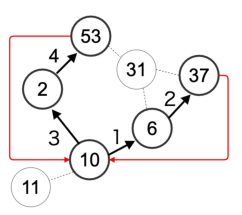
\includegraphics[width=7cm]{./figure/sequential-rw.pdf}
  \caption{1→4 の順にノードを移動しグラフを取得}
  \label{sequential-rw}
\end{figure}
\begin{figure}[t]
  \centering
  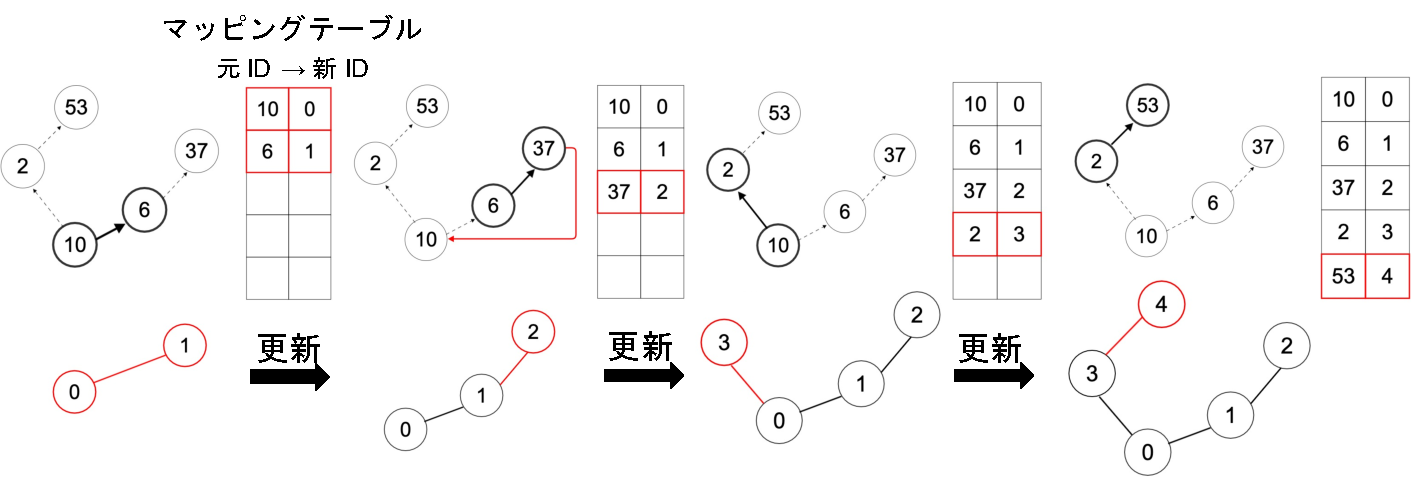
\includegraphics[width=\linewidth]{./figure/sequential.pdf}
  \caption{Sequential におけるノード ID 再配置}
  \label{sequential}
\end{figure}

\subsection{メモリ使用量を抑えたグラフ構造の保持}
Sequential では RW でノードを移動する度にマッピングテーブルの参照・登録及び再配置済みグラフの更新を行うことで
再配置待ちのグラフ構造を保持する必要を無くし,メモリ使用量を削減している.
図\ref{sequential_bad_memory}で示すように,グラフを取得してから再配置を行う場合は取得完了時のグラフと再配置済みのグラフを
メモリ上で保持する必要がある.
しかし,Sequential による再配置では図\ref{sequential_good_memory}で示すように,RW で移動した1エッジと再配置済みのグラフを保持するだけで良く,
1エッジを保持するためのメモリ使用量は取得完了時のグラフを保持するためのメモリ使用量より遥かに小さい.
\begin{figure}[t]
  \begin{tabular}{cc}
    \begin{minipage}[t]{0.45\hsize}
      \centering
      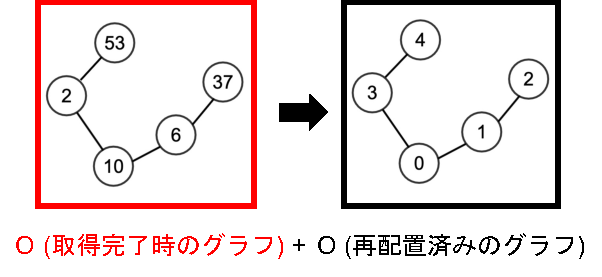
\includegraphics[width=7cm]{./figure/sequential_bad_memory.pdf}
      \caption{取得が完了してから再配置する場合の\\メモリ使用量}
      \label{sequential_bad_memory}
    \end{minipage} &
    \begin{minipage}[t]{0.45\hsize}
      \centering
      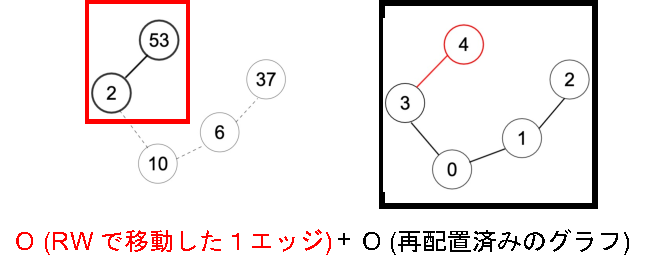
\includegraphics[width=7cm]{./figure/sequential_good_memory.pdf}
      \caption{Sequential において再配置に必要な\\メモリ使用量}
      \label{sequential_good_memory}
    \end{minipage}
  \end{tabular}
\end{figure}
\subsection{近接構造による局所性の部分的な実現}
Sequential は RW によるグラフ取得の途中で出会ったノード順に連続した ID を再配置するため ID の連続性は保証される.
さらに,RW では始点に戻る場合を除き,隣接ノードにしか移動しないため,図\ref{sequential-rw}で示す 1 → 2 のような移動の場合,
隣接ノードへ連続した ID が再配置される.
このように,Sequential では RW による移動の仕方によって隣接ノードへ連続した ID の再配置が可能となり,
近接構造によるアクセス局所性を考慮した再配置が部分的に実現されている.

\section{DBG Early Estimation (DBG-EE)}
DBG-EE では,RW によるグラフ取得の途中でノードを次数に基づきグループ分けし,各グループ毎に ID を再配置する.
なお,DBG-EE では DBG におけるグループ定義を踏襲し,グラフの平均次数$\mathbb{A}$に基づき,[0,$\mathbb{A}$/2),[$\mathbb{A}$/2,$\mathbb{A}$),[$\mathbb{A}$,2$\mathbb{A}$),[2$\mathbb{A}$,4$\mathbb{A}$),
[4$\mathbb{A}$,8$\mathbb{A}$),[8$\mathbb{A}$,16$\mathbb{A}$),[16$\mathbb{A}$,32$\mathbb{A}$),[32$\mathbb{A}$,$\infty$)
と 8 グループを定義する.
%ここで,高次数ノードが属する[32$\mathbb{A}$,$\infty$)側から順にグループ0,グループ1..,と名称を付けておく.
取得途中でノードをグループ分けし ID を再配置するには,予め各グループが再配置に使用する ID の範囲を定めておく必要がある.
そこで,DBG-EE では取得初期の段階で各グループのグループサイズを推定し,推定したサイズに基づいて各グループが再配置に使用する ID の範囲を決定する.
また,DBG-EE では取得途中で再配置を実行し,再配置済みのグラフへ反映が完了した時点で取得したグラフを破棄する.
これにより,取得完了まで再配置待ちのグラフを保持し続ける必要が無くなり,メモリ使用量が削減される.
さらに,グラフ取得と ID の再配置を並列して行うことで,グラフ取得を待つだけの時間が減少し,時間コストが削減される.
\subsection{グループサイズの早期推定}
全体で N 回 RW を実行する中で M 回毎に再配置を実行する場合,再配置は N/M 回実行される.
そこで,DBG-EE では1回目の再配置実行時のグループ分け結果に基づき各グループサイズを N/M 倍し,その値を各グループの推定サイズとみなす.
なお,グループ分けを実行する際には取得途中のグラフにおける平均次数を使用する.
図\ref{estimation_size} で示すように,1回目のグループ分けにより x 個のノードがグループ0へ割り振られた場合,グループ0の推定サイズは x $\times$ N/M となる.

\begin{figure}[t]
  \centering
  %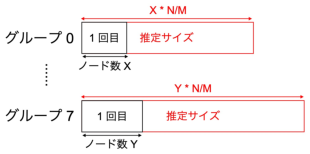
\includegraphics[width=\linewidth]{./figure/estimated_group_size.pdf}
  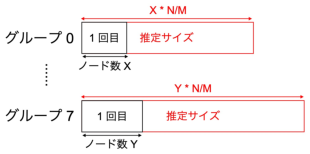
\includegraphics[width=10cm]{./figure/estimated_group_size.pdf}
  \caption{グループサイズの早期推定}
  \label{estimation_size}
\end{figure}
\subsection{推定サイズに基づく ID の範囲決定}
\begin{figure}[t]
  \centering
  %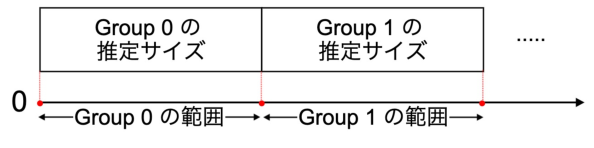
\includegraphics[width=\linewidth]{./figure/group_id_range.pdf}
  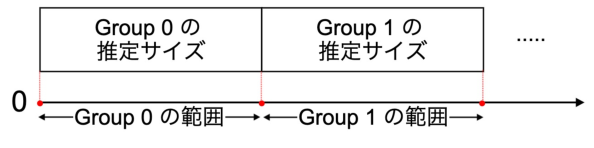
\includegraphics[width=10cm]{./figure/group_id_range.pdf}
  \caption{推定サイズに基づく ID の範囲決定}
  \label{degree_appro}
\end{figure}
\subsection{部分的な取得グラフの破棄}
\begin{figure}[t]
  \centering
  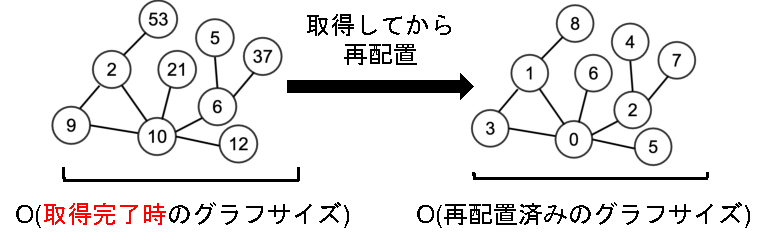
\includegraphics[width=\linewidth]{./figure/dbg-ee_bad_memory.pdf}
  \caption{取得途中のグラフと取得完了時のグラフにおける次数分布}
  \label{degree_appro}
\end{figure}
\begin{figure}[t]
  \centering
  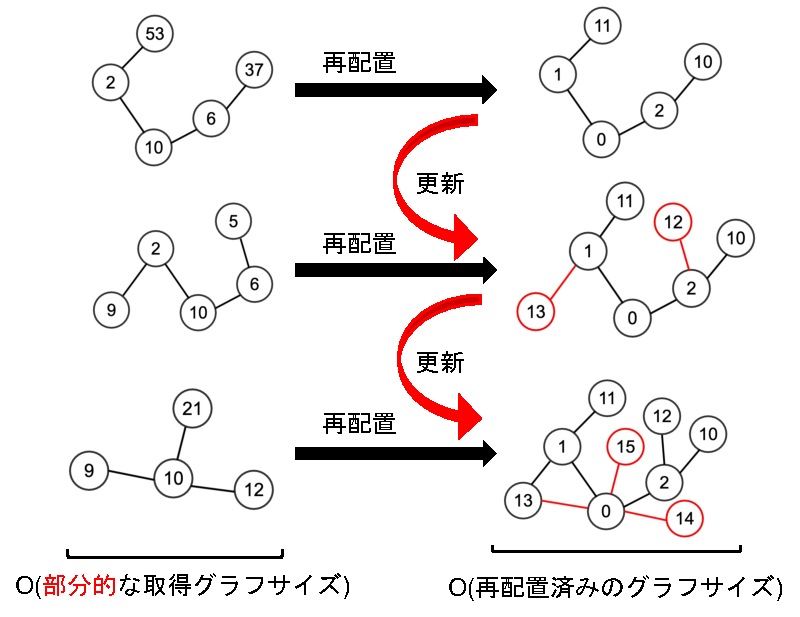
\includegraphics[width=\linewidth]{./figure/dbg-ee_good_memory.pdf}
  \caption{取得途中のグラフと取得完了時のグラフにおける次数分布}
  \label{degree_appro}
\end{figure}
\subsection{グラフ取得と再配置の並列処理}
\begin{figure}[t]
  \centering
  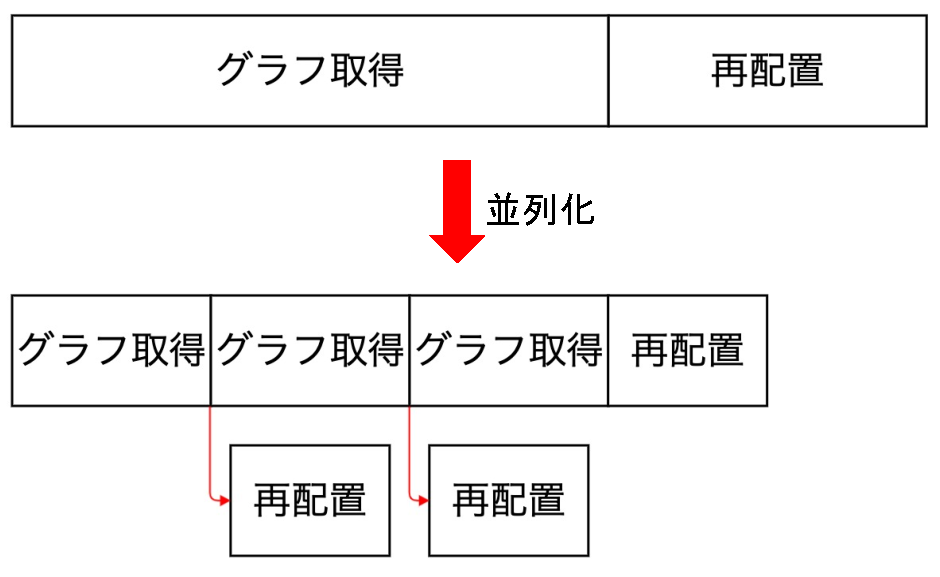
\includegraphics[width=\linewidth]{./figure/dbg-ee_para.pdf}
  \caption{取得途中のグラフと取得完了時のグラフにおける次数分布}
  \label{degree_appro}
\end{figure}